\documentclass[11pt]{article}
\usepackage[margin=0.75in]{geometry}
\usepackage{graphicx}
\pagestyle{empty}
\begin{document}
\begin{center}{\LARGE Odd-torsion translation proof review}\\[6pt]2026-11-03\end{center}
\noindent\textbf{Checked component.} Three independent joints support the abstract additive-law statement. A blind derivation gives $r(P+T)=T$ when $r$ is odd, $rP=0$, and $2T=0$; $T\ne0$ gives kernel exclusion. Explicit positive, even-scalar, and zero-$T$ controls test the hypotheses.\par\medskip
\noindent\textbf{Lean evidence.} The archived named hosted run passed its Torsion module build and zero-axiom audit. The downloaded receipt matches the frozen SHA-256 and complete input maps. Eleven hostile receipt mutations were rejected. The fresh current-head formal job was still running at reviewer freeze; an independent binary/kernel recheck was not performed.\par\medskip
\noindent\textbf{Verdict.} Semantic fidelity is faithful for the conditional additive statement. The archived machine result holds at byte-identical source scope. Full current-head validation remains inconclusive until the fresh formal result is checked. Concrete curve, point arithmetic, torsion certificate, and factor-base bridges remain separate.\par\medskip
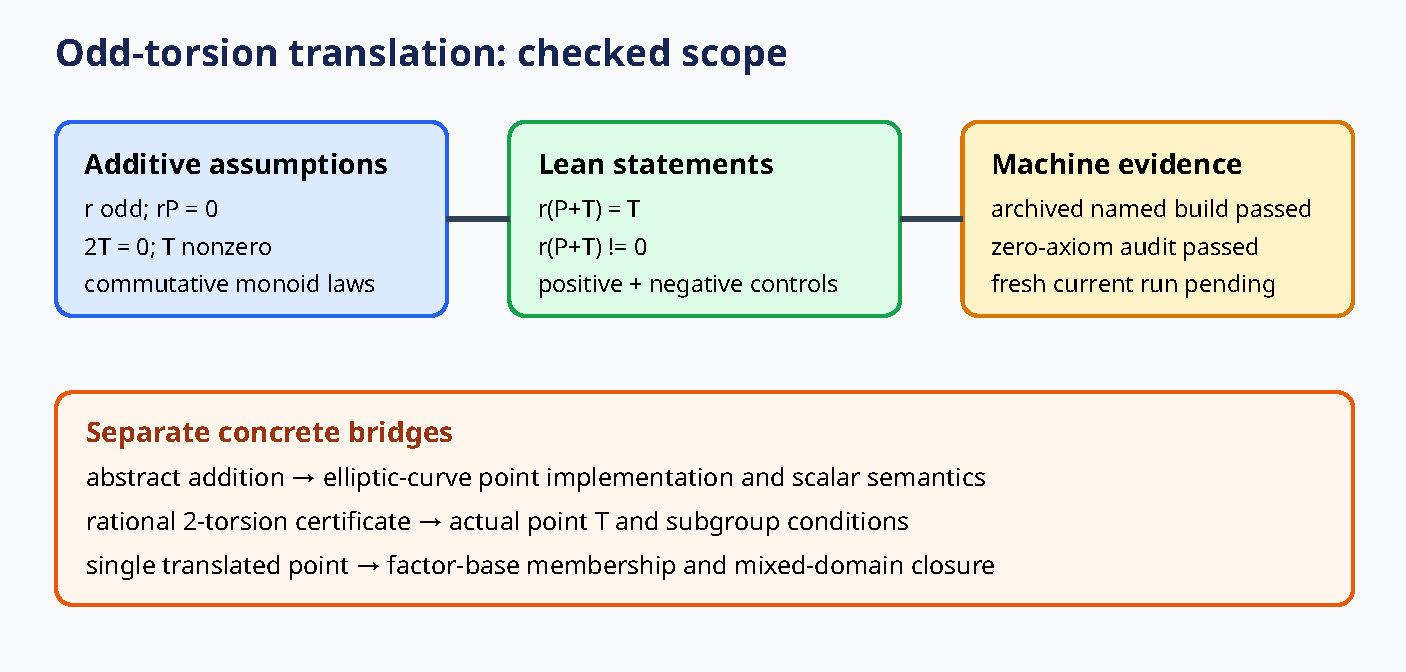
\includegraphics[width=\textwidth]{proof-boundary-figure.pdf}
\vfill\noindent\small Exact hashes, independent reports, the local Lean timeout, the older receipt mismatch, and the attestation-format adapter are preserved in REVIEW.md and reviews/.
\end{document}
